\documentclass[border=3pt]{standalone}
% Preâmbulo compartilhado pelos diagramas TikZ da aula 10 (Localização de Markov e Gaussiana)
\usepackage[T1]{fontenc}
\usepackage[utf8]{inputenc}
\usepackage{lmodern}
\usepackage{amsmath}
\usepackage{xcolor}
\usepackage{tikz}
\usetikzlibrary{arrows.meta,angles,quotes,decorations.pathmorphing,calc,
                positioning,shapes.geometric,shapes.misc,backgrounds,fit,
                math}

% Paleta (mesma dos SVGs originais)
\definecolor{dblue}{HTML}{2A5B8C}
\definecolor{dorange}{HTML}{B3541E}
\definecolor{dgreen}{HTML}{4A7C59}
\definecolor{dred}{HTML}{9C4B4B}
\definecolor{dcream}{HTML}{F4F1EA}
\definecolor{dshade}{HTML}{DDD7C9}

% Função gaussiana (não normalizada por padrão de escala visual)
\pgfmathdeclarefunction{gauss}{3}{%
  \pgfmathparse{1/(#3*sqrt(2*pi))*exp(-((#1-#2)^2)/(2*#3^2))}%
}

% Estilos comuns (prefixo d... para não colidir com chaves internas do pgf)
\tikzset{
  >={Stealth[length=2mm]},
  dguide/.style={gray!55, dashed, line width=0.4pt},
  daxis/.style={gray!60, line width=0.7pt, ->},
  dbody/.style={fill=black!3, draw=black!80, line width=1pt},
  dacc/.style={draw=dblue, line width=1pt},
  dlbl/.style={black!55, font=\small},
  dsub/.style={black!45, font=\footnotesize},
  dstate/.style={circle, draw=black!80, fill=dcream, line width=1pt,
                 minimum size=17mm, font=\large, inner sep=1pt},
  dobs/.style={circle, draw=black!80, fill=dshade, line width=1pt,
               minimum size=14mm, font=\large, inner sep=1pt},
  dbox/.style={rounded corners=2pt, draw=black!80, fill=dcream, line width=1pt,
               align=center, inner sep=6pt},
  dop/.style={circle, draw=black!80, fill=white, line width=1pt,
              minimum size=6mm, inner sep=0pt, font=\small},
  dtrans/.style={->, dblue, line width=1pt},
  dmeas/.style={->, dorange, line width=1pt},
  dcurve/.style={line width=1pt, dblue},
  dcurveb/.style={line width=1.4pt, dorange},
}

\usetikzlibrary{shapes.callouts}
\begin{document}
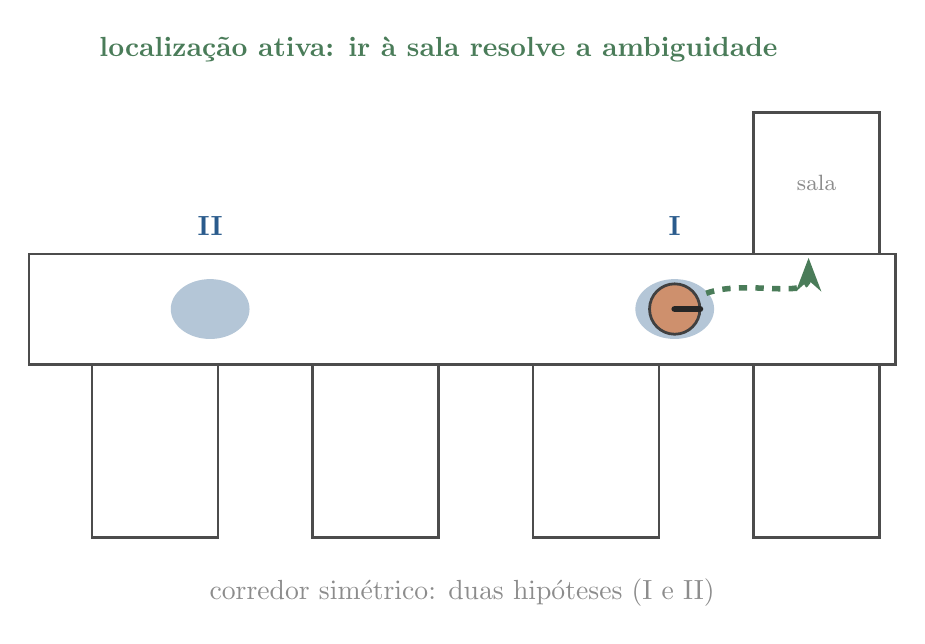
\begin{tikzpicture}[x=1cm,y=1cm,bal/.style={rectangle callout, rounded corners=7pt, draw=black!75, fill=white, line width=1pt, align=center, font=\normalsize, inner sep=5pt}]
  \newcommand{\robo}[3]{\begin{scope}[shift={(#1,#2)}, rotate=#3]\draw[black!75, fill=dorange!65, line width=1pt] (0,0) circle (0.32); \draw[black!85, line width=2.4pt, line cap=round] (0,0) -- (0.32,0);\end{scope}}

  \draw[black!70, fill=white, line width=1pt] (0,2.2) rectangle (11,3.6);
  \foreach \x in {1.6,4.4,7.2,10.0} {\draw[black!70, fill=white, line width=1pt] (\x-0.8,0) rectangle (\x+0.8,2.2);} 
  \draw[black!70, fill=white, line width=1pt] (9.2,3.6) rectangle (10.8,5.4);
  \node[font=\bfseries, dsub] at (10.0,4.5) {sala};
  \fill[dblue!35] (2.3,2.9) ellipse (0.5 and 0.38); \fill[dblue!35] (8.2,2.9) ellipse (0.5 and 0.38); \robo{8.2}{2.9}{0}
  \node[dblue, font=\normalsize\bfseries] at (2.3,3.95) {II}; \node[dblue, font=\normalsize\bfseries] at (8.2,3.95) {I};
  \draw[dgreen, line width=2pt, dashed, -{Stealth}] (8.6,3.1) to[out=20,in=270] (9.9,3.55);
  \node[dgreen, font=\normalsize\bfseries, align=center] at (5.2,6.2) {localização ativa: ir à sala resolve a ambiguidade};
  \node[dsub, font=\normalsize] at (5.5,-0.7) {corredor simétrico: duas hipóteses (I e II)};
\end{tikzpicture}
\end{document}
